% !Mode:: "TeX:UTF-8"
\chapter{SLAM: Present and Future}
\begin{mdframed}  
	\textbf{Goal of Study}
	\begin{enumerate}[labelindent=0em,leftmargin=1.5em]
		\item Understand the classic SLAM implementation scheme.
		\item Through experiments, compare the similarities and differences of various SLAM solutions.
		\item Explore the future development direction of SLAM.
	\end{enumerate}
\end{mdframed}

The working principle of each module in a SLAM system was introduced above, which is the crystallization of the work of researchers for many years. At present, in addition to these theoretical frameworks, we have also accumulated many excellent open source SLAM solutions. However, since most of their implementations are more complicated and not suitable for beginners' hands-on materials, we put them at the end of the book to introduce them. I believe that readers should be able to understand the basic principles by reading the previous content.

\newpage
\section{Open-source Implementations}
This lecture is a summary of the book. We will take readers to see how far the existing SLAM solutions can be. In particular, we focus on solutions that provide open source implementations. In the field of SLAM research, it is not easy to see open source solutions. Often the theories introduced in the paper only account for 20\% of the content, and the other 80\% are in the code, which is not mentioned in the paper. It is the selfless dedication of these researchers that has promoted the rapid advancement of the entire SLAM industry and enabled subsequent researchers to have a higher starting point. Before we start to do SLAM, we should have an in-depth understanding of similar solutions, and then conduct our own research, which will make more sense.

The first half of this lecture will lead the readers to take a tour of the current visual SLAM program and comment on its historical status, advantages and disadvantages. \autoref{table:opensource-slam}~ lists some popular open source SLAM solutions, and readers can choose the solutions they are interested in for research and experimentation \footnote{The book is basically written in 2016 so we cannot list the newer systems after 2016.}. Due to space limitations, we only selected a part of the representative plan, which is certainly not comprehensive. In the second half, we will explore some possible future development directions and give some current research results.

{
	\begin{table}[!h]
		\small
		\caption{Open source SLAM systems}
		\label{table:opensource-slam}
		\begin{tabu}{@{}c|c|X@{}}
			\toprule
			Name & Sensors & URL \\
			\midrule
			MonoSLAM &  M & \url{https://github.com/hanmekim/SceneLib2}  \\ 
			PTAM & M & \url{http://www.robots.ox.ac.uk/~gk/PTAM/} \\ 
			ORB-SLAM & M/S/R & \url{http://webdiis.unizar.es/~raulmur/orbslam/} \\ 
			LSD-SLAM & M & \url{http://vision.in.tum.de/research/vslam/lsdslam} \smallskip \\
			SVO & M & \url{https://github.com/uzh-rpg/rpg_svo} \\ 
			DTAM & R & \url{https://github.com/anuranbaka/OpenDTAM} \\ 
			DVO & R & \url{https://github.com/tum-vision/dvo_slam} \\ 
			DSO & M & \url{https://github.com/JakobEngel/dso} \\
			VINS & M+IMU & \url{https://github.com/HKUST-Aerial-Robotics/VINS-Mono} \\
			RTAB-MAP & S/R & \url{https://github.com/introlab/rtabmap} \\ 
			RGBD-SLAM-V2 & R & \url{https://github.com/felixendres/rgbdslam_v2} \\ 
			Elastic Fusion & R & \url{https://github.com/mp3guy/ElasticFusion} \\ 
			Hector SLAM & L & \url{http://wiki.ros.org/hector_slam} \\ 
			GMapping & L & \url{http://wiki.ros.org/gmapping} \\ 
			OKVIS & M/S+IMU & \url{https://github.com/ethz-asl/okvis} \\ 
			ROVIO & M+IMU & \url{https://github.com/ethz-asl/rovio} \\ 
			\bottomrule
		\end{tabu}
	\end{table}
}

\subsection{MonoSLAM}
When it comes to visual SLAM, the first thing that many researchers think of is A. J. Davison's monocular SLAM work {\cite{Davison2007,Davison2003}}. Professor Davison is a pioneer in the field of visual SLAM research. He proposed MonoSLAM in 2007 as the first real-time monocular visual SLAM system {\cite{Davison2007}}, which is considered the birthplace of many work. MonoSLAM uses the extended Kalman filter as the back end to track very sparse feature points on the front end. Since EKF occupies an obvious dominant position in early SLAM, MonoSLAM is also based on EKF, using the current state of the camera and all landmark points as the state quantity, and updating its mean and covariance.

\autoref{fig:mono-slam}~ shows the situation of MonoSLAM at runtime. It can be seen that the monocular camera tracks very sparse feature points in an image (and active tracking technology is used). In EKF, the position of each feature point obeys Gaussian distribution, so we can express its mean value and uncertainty in the form of an ellipsoid. In the right half of the picture, we can find some small balls distributed in space. The longer they appear in a certain direction, the more uncertain their position in that direction. We can imagine that if a feature point converges, we should be able to see it change from a very long ellipsoid (very uncertain in the direction of the camera $Z$) to a small point.

\begin{figure}[!htp]
	\centering
	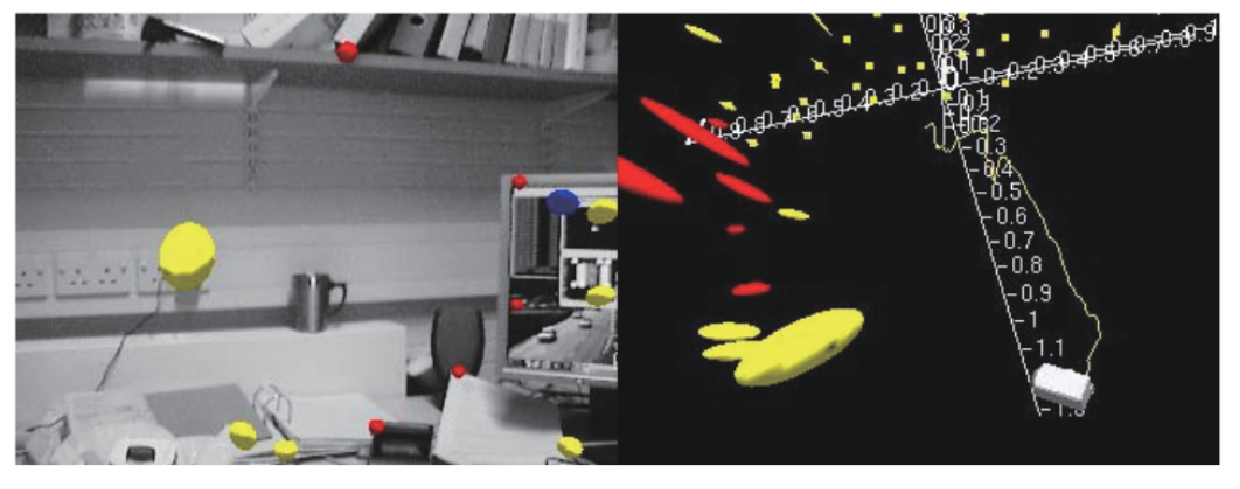
\includegraphics[width=1.0\textwidth]{past-and-future/mono-slam.pdf}
	\caption{Snapshot of MonoSLAM. Left: the tracked features. Right: the map point in 3D space.}
	\label{fig:mono-slam}
\end{figure}

This approach seems to have many drawbacks today, but it was already a milestone work at that time, because the previous visual SLAM system basically could not run online, and only rely on the robot to carry the camera to collect data, and then perform offline positioning. And build maps. The advancement of computer performance and the use of sparse methods to process images have combined to make a SLAM system run online. From a modern point of view, MonoSLAM has conditions such as narrow application scenarios, limited number of road signs, and sparse feature points that are very easy to lose. Its development has also been stopped and replaced by more advanced theories and programming tools. But this does not prevent us from understanding and respecting the work of our predecessors.

\subsection{PTAM}
In 2007, Klein's team proposed PTAM (Parallel Tracking and Mapping) {\cite{Klein2007}}, which is also an important event in the development of visual SLAM. The important significance of PTAM lies in the following two points:
\begin{enumerate}
	\item PTAM proposed and realized the parallelization of the tracking and mapping process. It is now clear that the tracking part needs to respond to image data in real time, and the optimization of the map does not need to be calculated in real time. Back-end optimization can be done slowly in the background, and then thread synchronization can be performed when necessary. This is the first time the concept of front and back ends have been distinguished in visual SLAM, leading to the design of many later visual SLAM systems (most of the SLAMs we see now are divided into front and back ends).
	\item PTAM is the first solution that uses nonlinear optimization instead of using traditional filters as the backend. It introduces a key frame mechanism: we don't need to process each image carefully, but string together several key images, and then optimize its trajectory and map. Early SLAM mostly used EKF filters or their variants, as well as particle filters. After PTAM, visual SLAM research gradually turned to the back end dominated by nonlinear optimization. Because people did not realize the sparsity of back-end optimization before, they felt that the optimized back-end could not process such large-scale data in real time, and PTAM is a significant counterexample.
	
	\hspace{2em}PTAM is also an augmented reality software that demonstrates cool AR effects (as shown in \autoref{fig:ptam}). According to the camera pose estimated by PTAM, we can place a virtual object on a virtual plane, which looks like it is in a real scene.
\end{enumerate}

\begin{figure}[!ht]
	\centering
	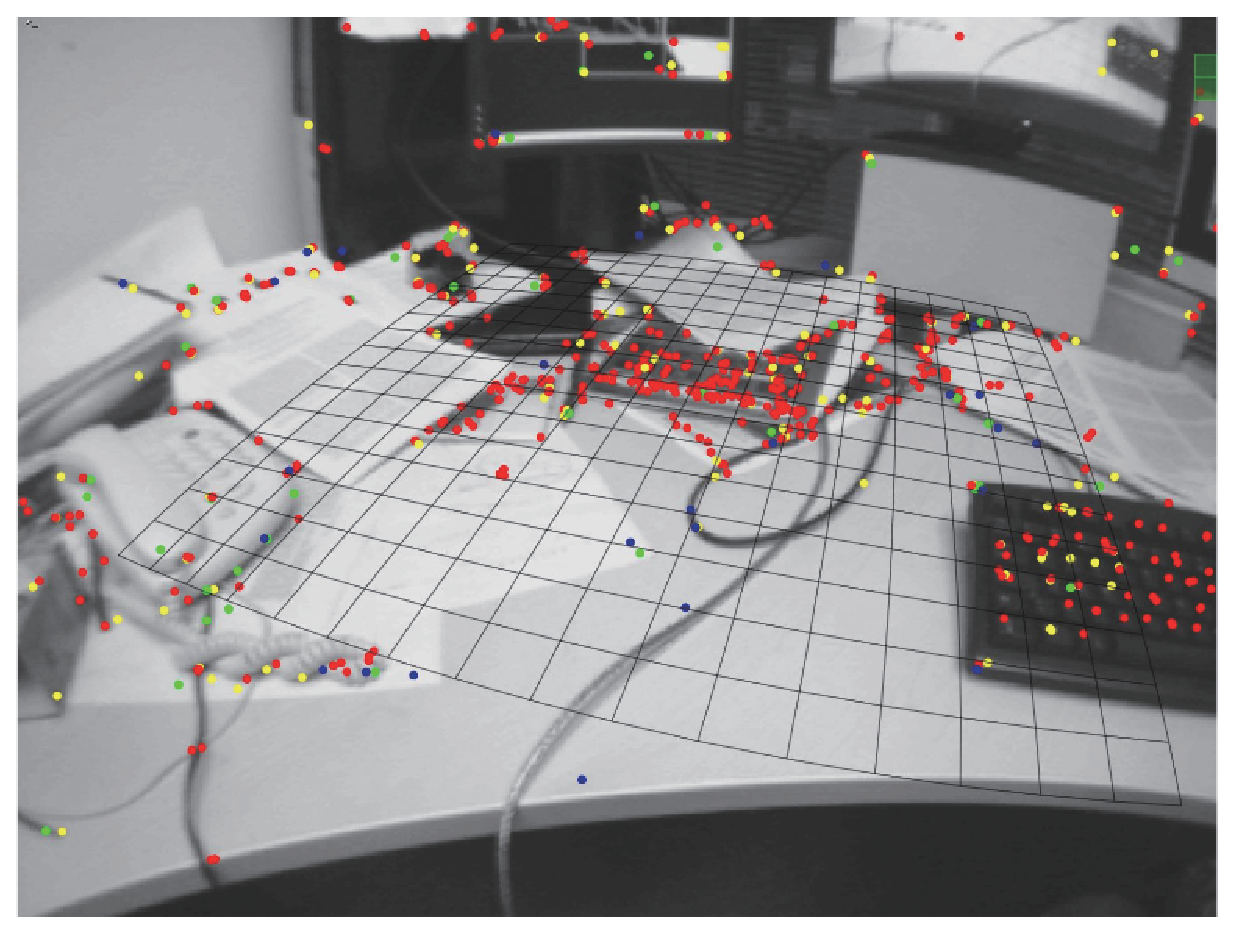
\includegraphics[width=1.0\textwidth]{past-and-future/ptam}
	\caption{Screenshot of PTAM demo. It can not only provide real-time SLAM functions, but also superimpose virtual objects on a virtual plane.}
	\label{fig:ptam}
\end{figure}

However, from a modern point of view, PTAM can be regarded as one of the early SLAM work combined with AR. Similar to many earlier works, there are obvious flaws: the scene is small, tracking is easy to lose, and so on. These were revised in the follow-up plan.

\subsection{ORB-SLAM Series} 
After introducing several historical solutions, let's look at some modern SLAM systems. ORB-SLAM is a very famous \textsuperscript{\cite{Mur-Artal2015}} among the successors of PTAM (see \autoref{fig:orb-slam}). It was proposed in 2015 and is one of the most complete and easy-to-use systems in modern SLAM systems (if not the most complete and easy-to-use). ORB-SLAM represents a peak of the mainstream feature point SLAM. Compared with previous work, ORB-SLAM has the following obvious advantages:

\begin{figure}[!ht]
	\centering
	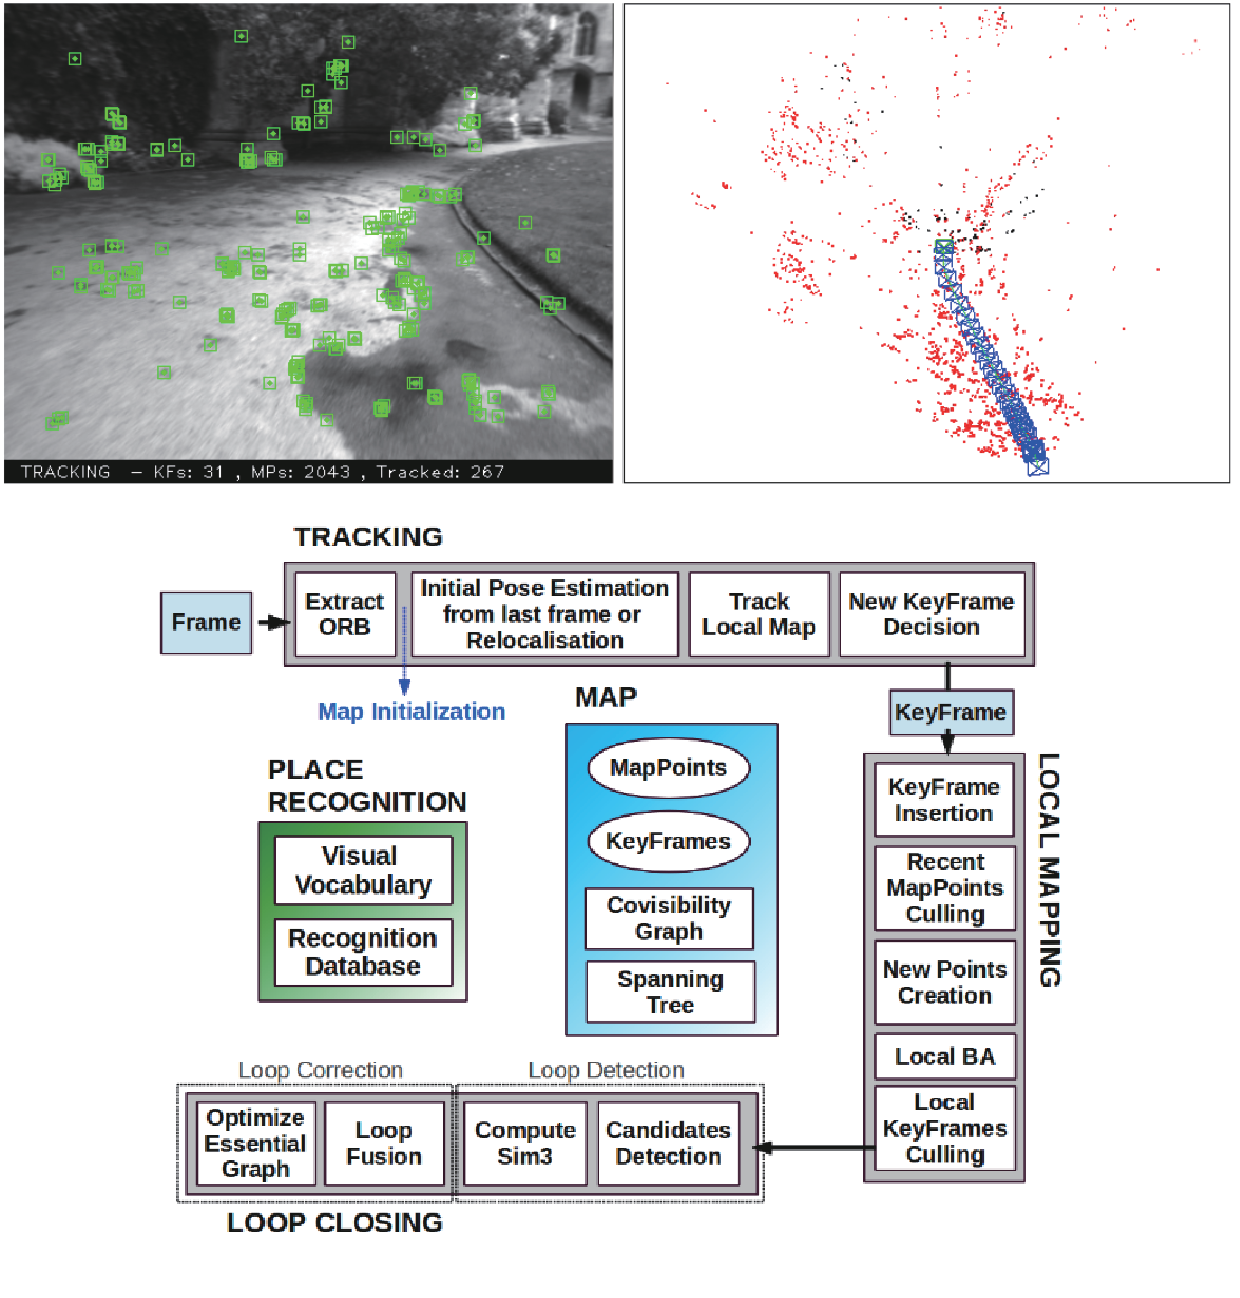
\includegraphics[width=1.0\textwidth]{past-and-future/orb-slam}
	\caption{ORB-SLAM running screenshot. The left side is the image and the tracked feature points, and the right side is the camera trajectory and the modeled feature point map. Below is the  three-thread framework.}
	\label{fig:orb-slam}
\end{figure}

\begin{enumerate}
	\item It supports three modes of monocular, binocular and RGB-D. This makes it possible to test it on ORB-SLAM, no matter what kind of common sensors we get, it has good versatility.
	\item The entire system is calculated around ORB features, including the ORB dictionary for visual odometry and loop detection. It reflects that the ORB feature is an excellent compromise between efficiency and accuracy of the computing platform at this stage. ORB is not as time-consuming as SIFT or SURF, and can be calculated in real time on the CPU; compared to simple corner features such as Harris corners, it has good rotation and scaling invariance. In addition, ORB provides descriptors that enable us to perform loop detection and relocation in a large range of motion.
	\item ORB's loop detection is its highlight. The excellent loopback detection algorithm ensures that ORB-SLAM effectively prevents accumulated errors and can be quickly retrieved after loss. Many existing SLAM systems are not perfect. For this reason, ORB-SLAM must load a large ORB dictionary \mbox{file}\footnote{Currently, the open source version of ORB-SLAM uses a text format dictionary, which can speed up a lot after changing to a binary format dictionary. }.
	\item ORB-SLAM innovatively uses three threads to complete SLAM: Tracking thread for real-time tracking of feature points, optimization thread for local Bundle Adjustment (Co-visibility Graph, commonly known as \textbf{small graph}), and global pose graph loop detection and optimization thread (essential graph, commonly known as \textbf{big graph}). Among them, the Tracking thread is responsible for extracting ORB feature points for each new image, comparing it with the most recent key frame, calculating the location of the feature points and roughly estimating the camera pose. The small picture thread solves a Bundle Adjustment problem, which includes the feature points in the local space and the camera pose. This thread is responsible for solving more refined camera poses and spatial locations of feature points. However, only the first two threads have completed a better visual odometer. The third thread, the big picture thread, performs loopback detection on the global map and key frames to eliminate accumulated errors. Because there are too many map points in the global map, the optimization of this thread does not include map points, but only the pose map composed of camera poses.
	
	\hspace{2em} Following the two-thread structure of PTAM, the three-thread structure of ORB-SLAM has achieved very good tracking and mapping effects, which can ensure the global consistency of the trajectory and the map. This three-thread structure will also be recognized and adopted by subsequent researchers.
	\item ORB-SLAM has carried out many optimizations around feature points. For example, on the basis of OpenCV feature extraction, the uniform distribution of feature points is ensured. When optimizing the pose, a loop optimization method is used to obtain more correct matches, which is a more relaxed key frame selection strategy than PTAM. and many more. These small improvements make ORB-SLAM far more robust than other solutions: even for poor scenarios and poor calibration internal parameters, ORB-SLAM can work smoothly.
\end{enumerate}

The above-mentioned advantages make ORB-SLAM reach its peak in the feature point SLAM. Many research works use ORB-SLAM as the standard, or follow-up development based on it. Its code is known for being clear and easy to read, with perfect annotations, which can be further understood by later researchers.

Of course, ORB-SLAM also has some shortcomings. First of all, since the entire SLAM system uses feature points for calculation, we must calculate the ORB feature for each image, which is very time-consuming. The three-thread structure of ORB-SLAM also brings a heavier burden to the CPU, making it only able to operate in real time on the CPU of the current PC architecture, and it is difficult to transform to embedded devices. Secondly, the mapping of ORB-SLAM is sparse feature points, and there is no open storage and relocation function after reading the map (although it is not difficult in terms of implementation). According to our analysis in the mapping section, the sparse feature point map can only meet our needs for positioning, but cannot provide navigation, obstacle avoidance, interaction and many other functions. However, if we only use ORB-SLAM to deal with the positioning problem, it seems a bit too heavyweight. In contrast, some other programs provide a more lightweight positioning, allowing us to run SLAM on low-end processors, or allow the CPU to handle other tasks.

\subsection{LSD-SLAM}
LSD-SLAM (Large Scale Direct monocular SLAM) is a SLAM work {\cite{Engel2013, Engel2014}} proposed by J. Engel et al. in 2014. Analogous to ORB-SLAM to feature points, LSD-SLAM marks the successful application of the monocular direct method in SLAM. The core contribution of LSD-SLAM is to apply the direct method to semi-dense monocular SLAM. Not only does it not need to calculate feature points, but it can also construct a semi-dense map-here semi-dense means mainly to estimate the pixel position with obvious gradient. Its main advantages are as follows:

\begin{enumerate}
	\item The direct method of LSD-SLAM is for pixels. The author creatively proposed the relationship between pixel gradient and direct method, and the angular relationship between pixel gradient and epipolar direction in dense reconstruction. These are discussed in Lecture 8 and Lecture 13 of this book. However, LSD-SLAM performs semi-dense tracking on monocular images, and the implementation principle is more complicated than the routines in this book.
	\item LSD-SLAM realizes the reconstruction of semi-dense scenes on the CPU, which is rarely seen in previous schemes. The method based on feature points can only be sparse, and most of the dense reconstruction schemes use RGB-D sensors, or use GPU to build dense maps\textsuperscript{\cite{Kerl2013}}. The TUM Computer Vision Group has realized this kind of real-time semi-dense SLAM on the CPU based on years of research on the direct method.
	\item I also said before that the semi-dense tracking of LSD-SLAM uses some subtle methods to ensure the real-time and stability of tracking. For example, LSD-SLAM does not use a single pixel or image block, but takes 5 points on the epipolar line at equal distances to measure its SSD; in depth estimation, LSD-SLAM first initializes the depth with random numbers, After the estimation, the depth mean is normalized to adjust the scale; when measuring the depth uncertainty, not only the geometric relationship of the triangle is considered, but also the angle between the epipolar line and the depth is considered, and it is summarized into a luminosity uncertainty item ; The constraints between key frames use the similar transformation group and the corresponding Lie algebra $\bm{\zeta} \in \mathfrak{sim}(3)$ to express the scale explicitly, which can be used in the back-end optimization Taking scenes of different scales into account, the scale drift phenomenon is reduced.
\end{enumerate}

\autoref{fig:lsd-slam}~ shows the operation of LSD. We can observe how this subtle semi-dense map is a form between the sparse map and the dense map. The semi-dense map models the parts with obvious gradients in the grayscale image. A large part of the map is displayed on the edges or textured parts of the object. LSD-SLAM tracks them and establishes key frames, and finally optimizes to get such a map. It seems that it has more information than a sparse map, but it does not have a complete surface like a dense map (dense maps are generally considered to be unable to achieve real-time performance with CPU alone).

\begin{figure}[!ht]
	\centering
	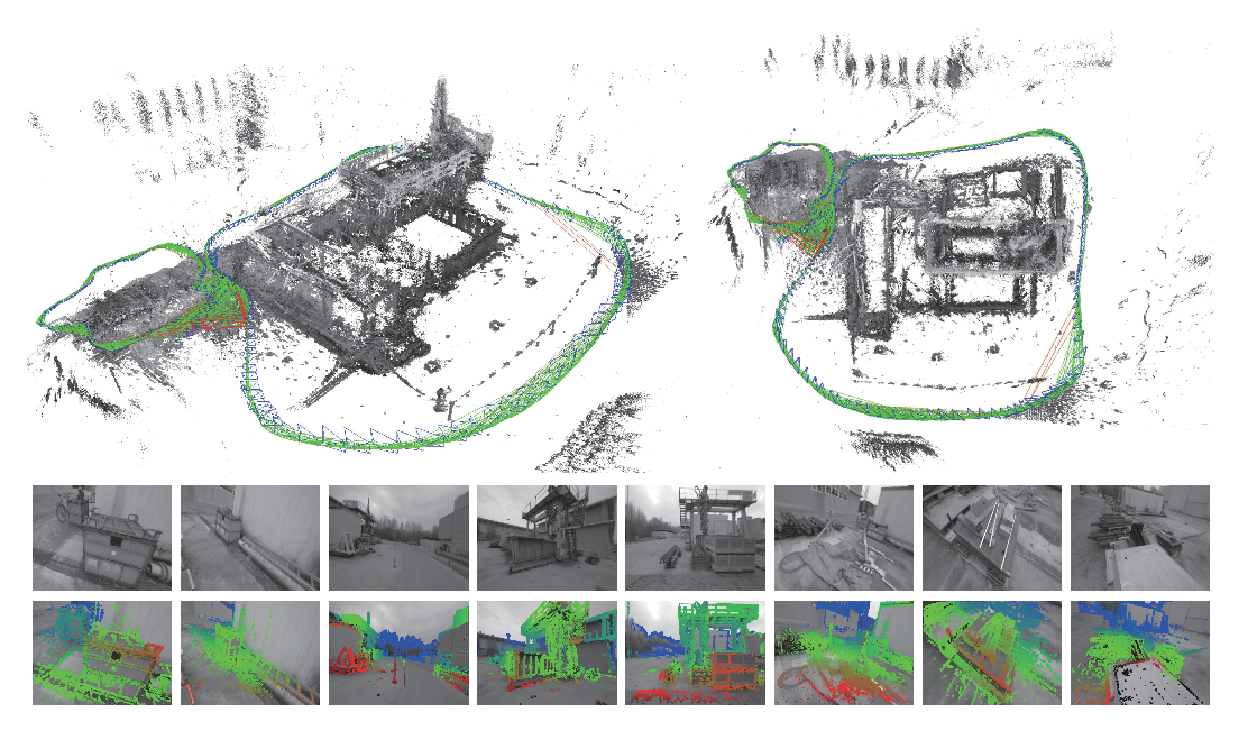
\includegraphics[width=1.0\textwidth]{past-and-future/lsd-slam}
	\caption{Snapshots of LSD-SLAM. The upper part is the estimated trajectory and map, and the lower part is the reconstructed part of the image, that is, the part with better pixel gradient.}
	\label{fig:lsd-slam}
\end{figure}

Since LSD-SLAM uses the direct method for tracking, it not only has the advantages of the direct method (insensitive to feature missing areas), but also inherits the shortcomings of the direct method. For example, LSD-SLAM is very sensitive to camera internal parameters and exposure, and is easily lost when the camera moves quickly. In addition, in the loop detection part, since there is currently no loop detection method based on the direct method, LSD-SLAM must rely on the feature point method for loop detection, and has not completely got rid of the calculation of feature points.

\subsection{SVO}
SVO is the abbreviation of Semi-direct Visual Odoemtry \textsuperscript{\cite{Forster2014}}. It is a visual odometer based on the sparse direct method proposed by Forster et al. in 2014. According to the author's name, it should be called the "semi-direct" method, but according to the conceptual framework of this book, it may be better to call it the "sparse direct method". The meaning of \textbf{semi-direct} in the original text refers to the mixed use of feature points and direct methods: SVO tracks some key points (corner points, no descriptors), and then, like the direct method, based on the information around these key points Estimate camera movement and its position (as shown in \autoref{fig:lsd-slam}). In implementation, SVO uses small blocks of $4\times4$ around the key points for block matching to estimate the camera's own motion.

Compared with other programs, SVO's biggest advantage is extremely fast. Due to the use of the sparse direct method, it does not have to laboriously calculate the descriptor, nor does it need to process as much information as dense and semi-dense, so it can achieve real-time performance even on low-end computing platforms, while on PC platforms It can reach a speed of more than 100 frames per second. In the subsequent SVO 2.0, the speed has reached an astonishing 400 frames per second. This makes SVO very suitable for occasions with limited computing platforms, such as the positioning of drones and handheld AR/VR devices. UAV is also the target application platform for the author to develop SVO.


\begin{figure}[H]
	\centering
	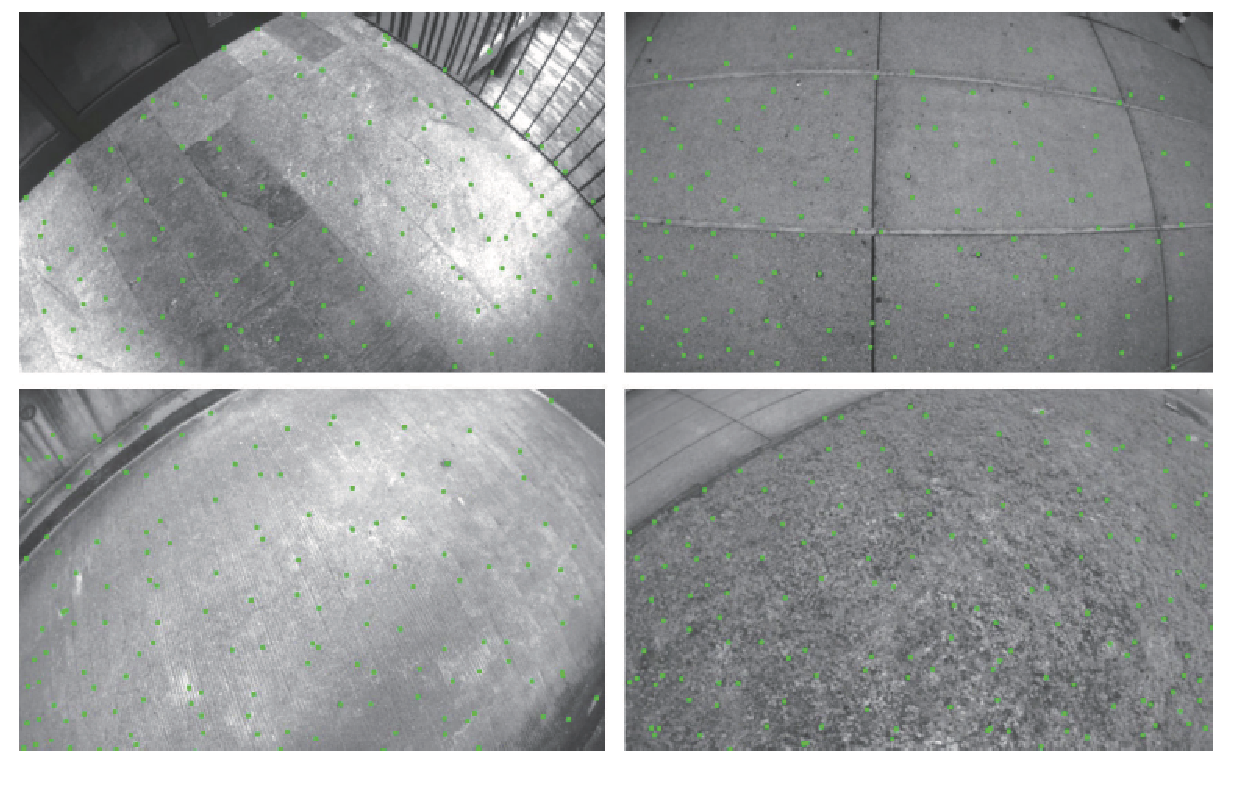
\includegraphics[width=1.0\textwidth]{past-and-future/svo}
	\caption{Features tracked by SVO.}
	\label{fig:svo}
\end{figure}

Another innovation of SVO is that it puts forward the concept of depth filter and derives a depth filter based on uniform-Gaussian mixture distribution. This is mentioned in Lecture 13 of this book, but since the principle is more complicated, we did not explain it in detail. SVO uses this filter to estimate the position of key points, and uses the inverse depth as a parameterized form to better calculate the position of feature points.

The open source version of SVO code is clear and easy to read, which is very suitable for readers to analyze as the first SLAM example. However, the open source version of SVO also has some problems:
\begin{enumerate}
	\item Since the target application platform is the drone's top-down camera, the object in its field of view is mainly the ground, and the camera's movement is mainly horizontal and up-and-down movement. Many details of SVO are designed around this application, which makes its performance being not very good in head-up cameras. For example, SVO uses the decomposition of the $\bm{H}$ matrix instead of the traditional $\bm{F}$ or $\bm{E}$ matrix during monocular initialization, which requires the assumption that the feature points are on the plane on. This assumption is true for a top-down camera, but it is usually not true for a head-up camera, which may cause initialization failure. For another example, when SVO selects a key frame, it uses the translation amount as a strategy for determining a new key frame without considering the rotation amount. This is also effective in the drone's top view configuration, but it is easy to lose in the head-up camera. Therefore, if readers want to use SVO in a head-up camera, they must modify it themselves.
	\item SVO discards the back-end optimization and loop closure detection part for speed and light weight, and basically has no image building function. This means that SVO pose estimation must have cumulative errors, and it is not easy to relocate after loss (because there is no descriptor for loop detection). Therefore, we call it a VO, not a complete SLAM.
\end{enumerate}

\subsection{RTAB-MAP}
After introducing several monocular SLAM solutions, let's look at some SLAM solutions on RGB-D sensors. Compared with monocular and binocular, the principle of RGB-D SLAM is much simpler (though not necessarily in implementation), and it can build dense maps in real time on the CPU.

RTAB-MAP (Real Time Appearance-Based Mapping) {\cite{Labbe2014}} is a more classic scheme in RGB-D SLAM. It implements everything that should be in RGB-D SLAM: feature-based visual odometry, bag-of-words-based loop detection, back-end pose map optimization, and point cloud and triangular mesh maps. Therefore, RTAB-MAP provides a complete (but somewhat huge) RGB-D SLAM solution. At present, we can obtain the binary program directly from ROS. In addition, the App can also be used on Google Project Tango (as shown in \autoref{fig:rtabmap}~)。

\begin{figure}[!ht]
	\centering
	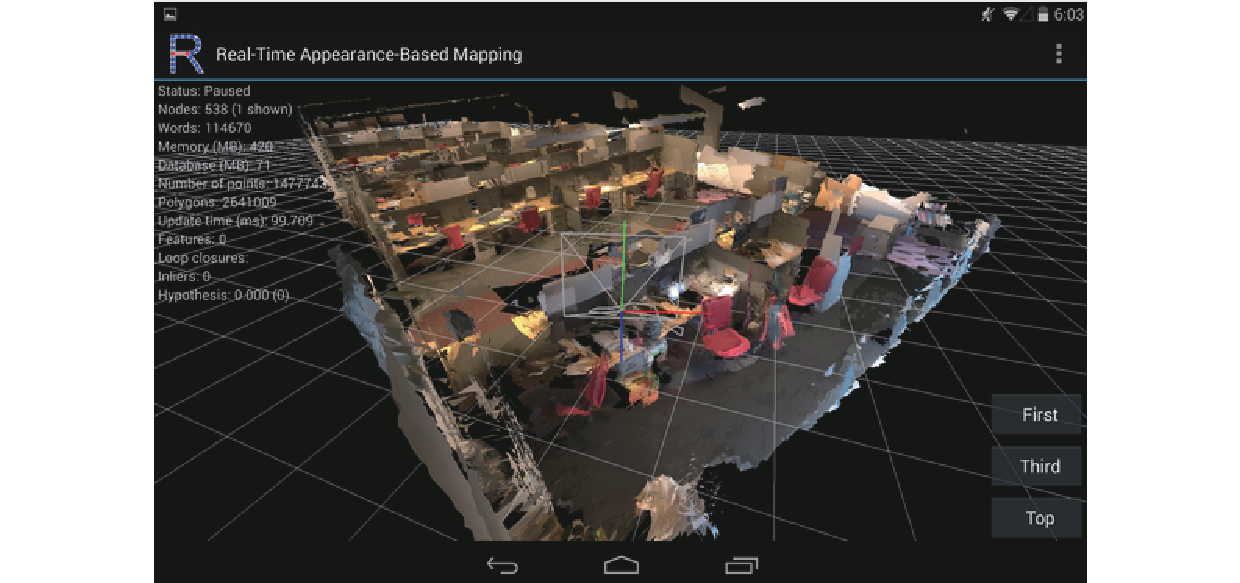
\includegraphics[width=1.0\textwidth]{past-and-future/rtabmap}
	\caption{RTAB-MAP in Google Project Tango.}
	\label{fig:rtabmap}
\end{figure}

RTAB-MAP supports some common RGB-D and binocular sensors, such as Kinect, Xtion, etc., and provides real-time positioning and mapping functions. However, due to the high level of integration, it becomes difficult for other developers to carry out secondary development based on it, so RTAB-MAP is more suitable for SLAM applications rather than research use.

\subsection{Others}
In addition to these open source solutions, readers can also find many other studies on websites such as \url{openslam.org}, for example, DVO-SLAM {\cite{Kerl2013a}}, RGBD-SLAM-V2 {\cite{Endres2014}}, DSO  {\cite{Engel2016}}, and some Kinect Fusion related work, etc. With the development of the times, newer and better open source SLAM works will also appear in people's field of vision. Due to space limitations, I will not introduce them one by one here.

\section{SLAM in Future}
After reading the existing systems, let’s discuss some future development directions\footnote{Well, this part is my personal understanding, which may not be completely correct.}. Generally speaking, the future development trend of SLAM is divided into two categories: one is to develop towards lightweight and miniaturization, so that SLAM can run well on small devices such as embedded or mobile phones, and then consider applications that use it as the underlying function. . After all, in most cases, our real goal is to realize the functions of robots and AR/VR devices, such as sports, navigation, teaching, and entertainment. SLAM is to provide its own pose estimation for upper-level applications. In these applications, we do not want SLAM to occupy all computing resources, so there is a very strong demand for the miniaturization and lightweight of SLAM. On the other hand, it uses high-performance computing equipment to realize functions such as precise 3D reconstruction and scene understanding. In these applications, our goal is to reconstruct the scene perfectly, and there are no restrictions on the portability of computing resources and equipment. Since GPU can be used, this direction and deep learning also have a combination.

\subsection{IMU Integrated VSLAM}
First, we want to talk about a direction with a strong application background: the visual-inertial navigation fusion SLAM scheme. Whether actual robots or hardware devices, they usually do not only carry one sensor, but are often a fusion of multiple sensors. Researchers in academia love the \textit{big clean problems}, such as implementing visual SLAM with a single camera. But friends in the industry pay more attention to making algorithms more practical and have to face some complex and trivial scenarios. In this application context, the use of vision and inertial navigation to integrate SLAM has become a hot spot.

The inertial sensor (IMU) can measure the angular velocity and acceleration of the sensor body, which is considered to have obvious complementarity with the camera sensor, and has the potential to obtain a more complete SLAM system after fusion {\cite{Gui2015}}. Why do we say that?

\begin{enumerate}
	\item IMU can measure angular velocity and acceleration, but these quantities have obvious drift (Drift), which makes the pose data obtained by integration twice very unreliable. For example, if we put the IMU on the table without moving, the posture obtained by integrating its readings will drift out of the distance. However, for fast movements in a short period of time, IMU can provide some better estimates. This is the weakness of the camera.
	
	When the movement is too fast, the camera (rolling shutter) will have motion blur, or the overlapping area between two frames is too small to be able to perform feature matching, so pure visual SLAM is very afraid of fast movement. With IMU, we can maintain a better pose estimation even during the period when the camera data is invalid, which is not possible with pure visual SLAM.
	
	\item Compared with IMU, the camera data will basically not drift. If the camera is placed in place and fixed, then (in a static scene) the pose estimation of visual SLAM is also fixed. Therefore, the camera data can effectively estimate and correct the drift in the IMU reading, so that the pose estimation after slow motion is still valid.
	
	\item When the image changes, we essentially cannot know whether the camera itself has moved or the external conditions have changed, so pure visual SLAM is difficult to deal with dynamic obstacles. The IMU can feel its own motion information, to some extent reduce the impact of dynamic objects.
\end{enumerate}

In summary, we see that IMU provides a better solution for fast motion, and the camera can solve the drift problem of IMU under slow motion-in this sense, the two are complementary.

\begin{figure}[!thp]
	\centering
	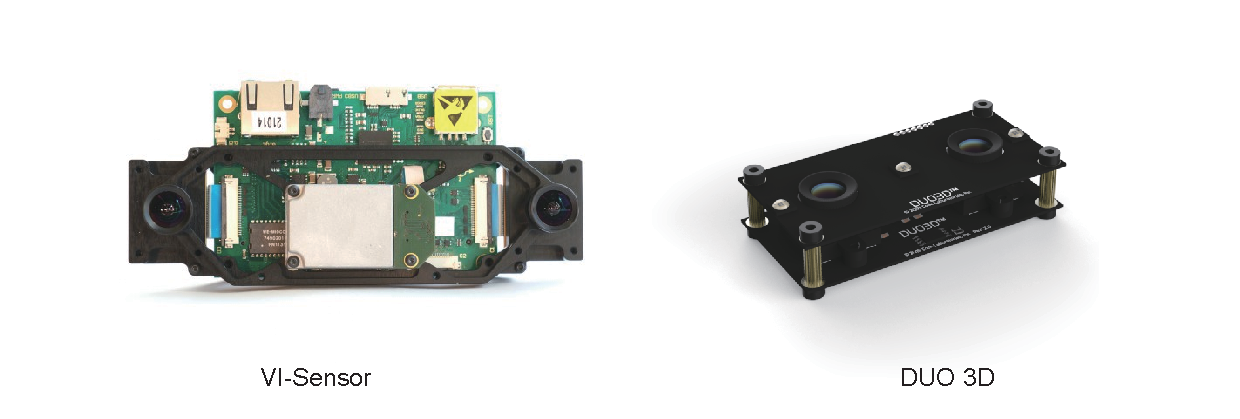
\includegraphics[width=1.0\textwidth]{past-and-future/visensor}
	\caption{More and more devices start to integrate IMU with cameras. }
	\label{fig:visensor}
\end{figure}

Of course, although it sounds very good, VIO (Visual Inertial Odometry) is quite complicated whether it is theory or practice. Its complexity mainly comes from the fact that IMU measures acceleration and angular velocity, so kinematic calculations have to be introduced. At present, the framework of VIO has been finalized into two categories: loosely coupled and tightly coupled {\cite{Martinelli2014}}. Loose coupling means that the IMU and the camera perform their own motion estimation separately, and then merge their pose estimation results. Tight coupling refers to combining the state of the IMU with the state of the camera, jointly constructing the motion equation and observation equation, and then performing state estimation-this is very similar to the theory we introduced before. We can foresee that tightly coupled theory will also be divided into two directions: filtering-based and optimization-based. In terms of filtering, the traditional EKF {\cite{Bloesch2015}} and the improved MSCKF (Multi-State Constraint KF) {\cite{Li2013}} have achieved certain results, and the researchers have also carried out the EKF In-depth discussion (such as observability {\cite{Huang2014}}); there are also corresponding solutions for optimization {\cite{Leutenegger2015, Forster2015}}. It is worth mentioning that although optimization methods in pure visual SLAM have taken the mainstream, in VIO, because the data frequency of IMU is very high, the amount of calculation required to optimize the state is greater, so it is still in filtering and Optimizing the coexistence stage {\cite{Tkocz2015, Usenko2016}}. Due to its complexity and limited space, I can only briefly introduce this direction here.

VIO provides a very effective direction for the miniaturization and cost reduction of SLAM in the future. And combined with the sparse direct method, we are expected to achieve good SLAM or VO effects on low-end hardware, which is very promising.

\subsection{Semantic SLAM}
Another general direction of SLAM is to combine with deep learning technology. So far, SLAM solutions are at the feature point or pixel level. We don't know what exactly these feature points or pixels come from. This makes the SLAM in computer vision not very similar to what we humans do, at least we never see the feature points, nor do we judge our own movement direction based on the feature points. We see objects one by one, judge their distance through the left and right eyes, and then guess the movement of the camera based on their movement in the image.

A long time ago, researchers tried to incorporate object information into SLAM. For example, the literature \cite{Nuechter2008, Civera2011, Koppula2011, Anand2012} once combined object recognition and visual SLAM to construct a map with object labels. On the other hand, by introducing the label information into the objective function and constraints of the BA or optimization end, we can combine the position of the feature point with the label information to optimize {\cite{Fioraio2013}}. These tasks can be called semantic SLAM. In summary, the combination of SLAM and semantics mainly has two aspects {\cite{Cadena2016}}:

\begin{enumerate}
	\item Semantics help SLAM. Traditional object recognition and segmentation algorithms often only consider one image, while in SLAM we have a moving camera. If we put object labels on all the pictures during the movement, we can get a labeled map. In addition, object information can also bring more conditions for loop detection and BA optimization.
	\item SLAM helps semantics. Both object recognition and segmentation require a lot of training data. In order for the classifier to recognize objects from various angles, it is necessary to collect data of the object from different perspectives, and then perform manual calibration, which is very difficult. In SLAM, since we can estimate the movement of the camera, we can automatically calculate the position of the object in the image, saving the cost of manual calibration. If there is automatically generated sample data with high-quality annotations, it can greatly accelerate the training process of the classifier.
\end{enumerate}

\begin{figure}[!thp]
	\centering
	\includegraphics[width=1.0\textwidth]{past-and-future/semantic-slam}
	\caption{Semantic SLAM results from \cite{Anand2012, Salas-Moreno2014}.}
	\label{fig:semantic-slam}
\end{figure}

Before deep learning is widely used, we can only use traditional tools such as support vector machines and conditional random fields to segment and recognize objects or scenes, or directly compare observation data with samples in the database. {\cite{Salas- Moreno2013, Salas-Moreno2014}}, try to build a semantic map {\cite{Anand2012, Stueckler2012, Kostavelis2013, Couprie2013}}. Because these tools themselves have limitations on the classification accuracy, the effect is often not satisfactory. With the development of deep learning, we began to use the network to recognize, detect and segment images more and more accurately {\cite{Deng2009, Krizhevsky2012, He2015, Ren2015, Long2014, Zheng2015}}. This lays a better foundation for constructing accurate semantic maps {\cite{Gupta2014}}. We are seeing that some scholars are gradually introducing neural network methods into the object recognition and segmentation in SLAM, and even the pose estimation and loop detection of SLAM itself {\cite{Konda2015, Kendall2015, Hou2015}}. Although these methods have not yet become mainstream, the combination of SLAM and deep learning to process images is also a promising research direction.

In addition, SLAM based on line/surface features  {\cite{An2012, Zhou2015, Benedettelli2012}} , SLAM in dynamic scenes {\cite{Saarinen2013, Maddern2012, Wang2008}}, and multi-robot SLAM {\cite{Zou2013, Gil2010a, Vidal-Calleja2011}}, etc., are all places where researchers are interested in concurrency. According to the opinion of the \cite{Cadena2016}, visual SLAM has gone through three major eras: asking questions, searching for algorithms, and improving algorithms. And we are currently in the third era, facing how to further improve the existing framework, so that the visual SLAM system can operate stably under various interference conditions. This step requires the unremitting efforts of many researchers.

Of course, no one can predict the future, and we are not sure if one day, the entire framework will be overturned and rewritten by new technologies. But even then, our contribution today will still be meaningful. Without today's research, there will be no future development. Finally, I hope that readers will have a full understanding of the entire existing SLAM system after reading this book. We also look forward to your contribution to SLAM research!

\section*{Exercises}
\begin{enumerate}
	\item Choose any of the open source SLAM systems mentioned in this lecture, compile and run it on your machine, and experience the process intuitively.
	\item You should be able to understand most SLAM related papers. Pick up paper and pen and start your research!
\end{enumerate}

